\pagebreak
\section{Foundations for the Operational Fit Dimension}
\label{sec:foundations-operational-fit}

The Operational Fit dimension addresses three runtime concerns that interact tightly: how modules survive extraction across a network boundary (G4), how the deployment pipeline supports both monolith and extracted-service topologies (G5), and how observability remains coherent across both deployment shapes (G6). The three guidelines share two foundational concepts that this section introduces before the per-guideline content. The first is the structural shift from an in-process boundary to a network boundary that gives the dimension its coherence: every Operational Fit guideline addresses one aspect of what happens when a module crosses that boundary. The second is the saga coordination pattern, the most consequential mechanism that all three guidelines depend on for handling cross-module workflows under distributed failure.

\subsection*{The In-Process to Network Boundary}
\label{sec:foundations-op-fit-network-boundary}

The Operational Fit guidelines share a common architectural concern: how a modular monolith survives the transition from a co-located deployment to a distributed one when a module is extracted as an independent service. Inside the monolith, modules communicate through method calls and share infrastructure: database connections, in-process event buses, runtime memory. When a module crosses the network boundary, every assumption that held in-process becomes a runtime concern. Latency replaces instantaneous calls. Partial failure replaces the certainty of in-process exceptions. Observability that was implicit in a single process becomes a coordination problem across services.

Three operational characteristics of the transition shape G4, G5, and G6 respectively.

\paragraph*{Consistency.} In-process modules can rely on database transactions for atomic cross-module operations; the network boundary makes this impossible. G4 addresses this by replacing implicit transactional consistency with the saga pattern, where cross-module workflows become compensable sequences that survive partial failure. Section~\ref{sec:g4-saga-styles} develops the saga coordination styles that operationalize this shift.

\paragraph*{Deployment topology.} In-process modules deploy as a single artifact; extracted services need independent build, deploy, and release pipelines without losing the ergonomics of working in a single repository. G5 addresses this through a deployment spectrum (D0 to D2) that lets the monolith deploy as one unit at first and adds deployment targets only when extraction is warranted.

\paragraph*{Observability continuity.} In-process modules can be monitored through a single set of logs, metrics, and traces; extracted services need distributed tracing through correlation identifiers that preserve the request flow across the network boundary. G6 addresses this by introducing the observability infrastructure (correlation identifiers, module-scoped metrics, structured logs) inside the monolith from inception, so that the same instrumentation continues to work after extraction without redesign.

The transition is not a single switch but a spectrum: G4, G5, and G6 provide the structural and operational scaffolding that lets a module move from full co-location to network independence without rewriting the system. The next subsection develops the most consequential coordination mechanism that all three guidelines depend on, the saga.

\subsection*{Saga Coordination Styles}
\label{sec:g4-saga-styles}

Saga coordination is the most consequential cross-cutting concept of the Operational Fit dimension. G4 builds on this section directly when prescribing the saga implementation; G5 and G6 assume that a saga choice has been made when the deployment topology and the observability requirements are specified. Both styles implement the same logical contract (a compensable cross-module workflow that survives partial failure); what separates them is where workflow control lives, how participants are coupled to each other, and which team topology each style assumes. The section develops each style with its own discussion and illustration, consolidates the contrast in a table, and closes with the trade-off that the per-guideline application of G4 Applied resolves for the Tiny Store.

\subsubsection*{Orchestrated saga}

An orchestrated saga places one component, an orchestrator, in charge of the entire sequence. The orchestrator calls each participating module in order, persists the workflow state, and triggers compensating actions on failure. Newman~\cite{newman2019monolith} describes this style as the closer analogue of the synchronous transaction it replaces: a single piece of code reads as the workflow, makes the sequencing explicit, and concentrates the failure-handling logic in one place. The orchestrator is typically implemented as a durable workflow engine, with Temporal, Camunda, and Zeebe as the practitioner references; the engine persists workflow state across process restarts, retries failed activities according to declarative policies, and runs compensating actions when an activity returns an unrecoverable failure.

The strength of the orchestrated style is its centralization. Richardson~\cite{richardson2018microservices} places the orchestrator at the head of a small set of patterns that distributed systems consistently rediscover for the same reason: when failure can occur at multiple steps, a single component that knows the full sequence is easier to operate than a graph of independent reactors. Newman~\cite{newman2019monolith} reinforces this view by observing that orchestrated sagas dominate in systems where one team owns the workflow end to end, because the team can change the orchestrator without coordinating with anyone. The cost, both authors note, is that the orchestrator can grow into a god-component if business logic creeps into it, and that every participant carries an implicit dependency on the orchestrator's contract. Khononov~\cite{khononov2024balancing} reads this concentration of coupling as a controlled trade rather than a structural failure, because the coupling stays within the boundary of the team that owns the orchestrator. Figure~\ref{fig:saga-orchestrated} shows the style as the Tiny Store implements it for the order fulfillment workflow: a central workflow engine drives each participating module in sequence and awaits a reply at every step.

\begin{figure}[H]
  \centering
  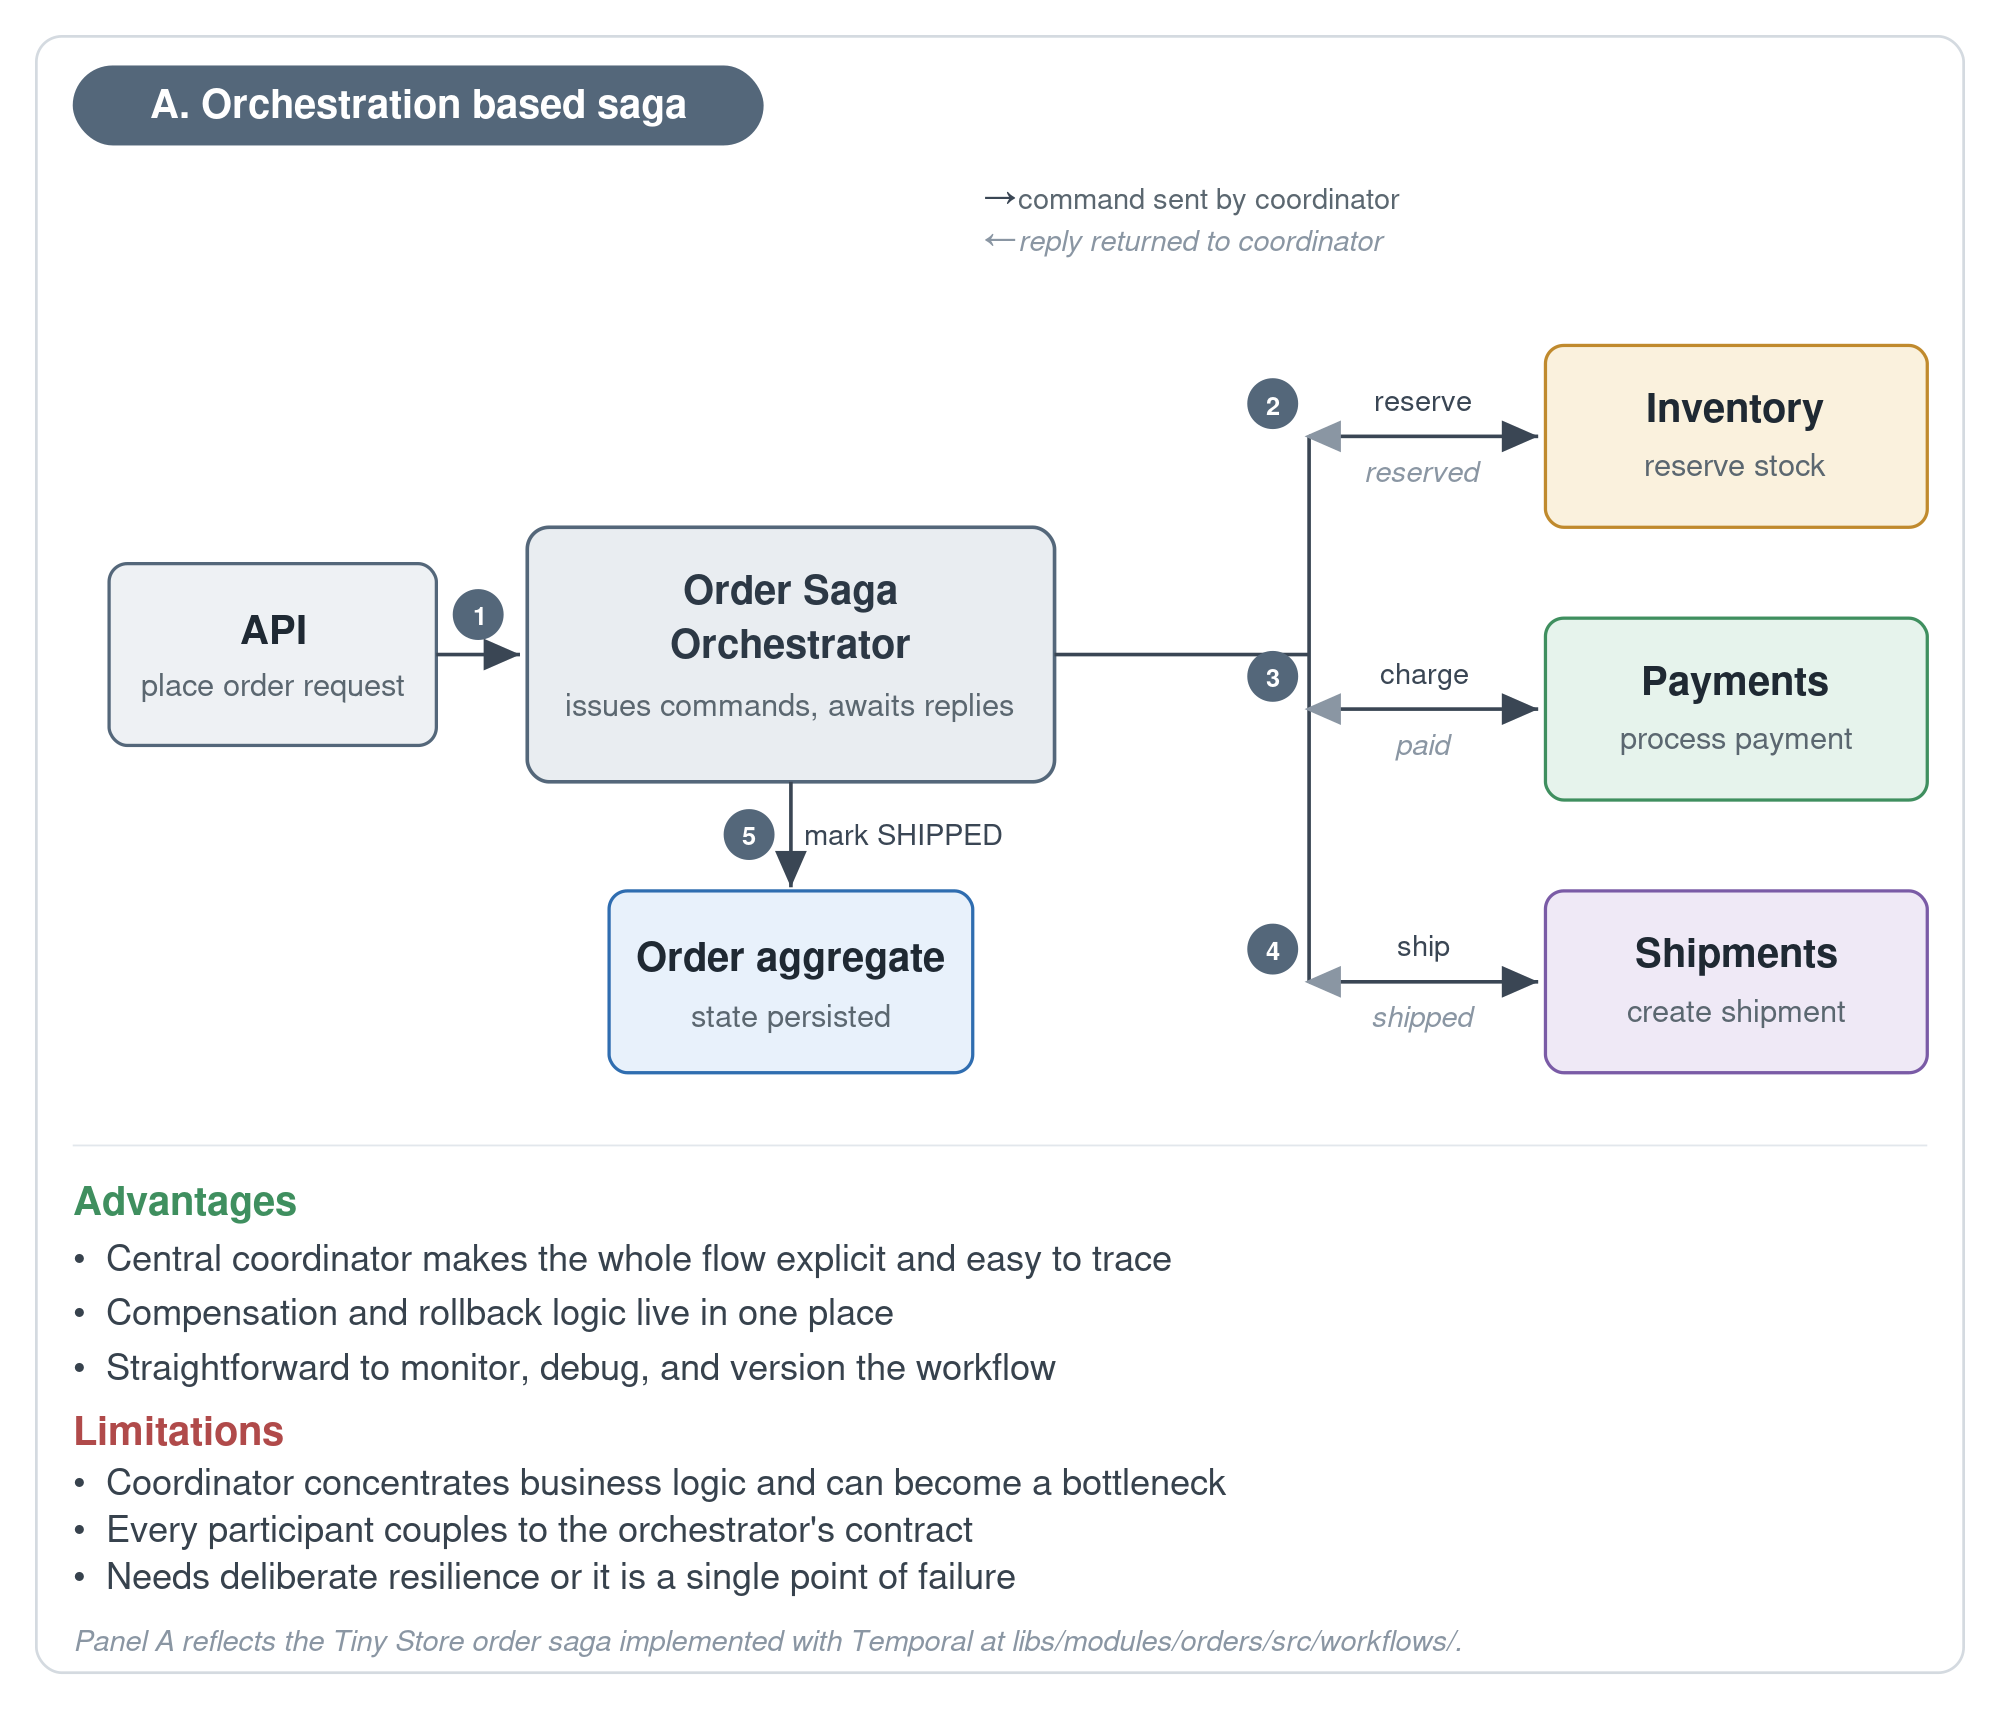
\includegraphics[width=\linewidth]{Cap4/guidelines/saga_pattern_A.png}
  \caption{Orchestrated saga style in the Tiny Store order fulfillment workflow}
  \label{fig:saga-orchestrated}
\end{figure}

\subsubsection*{Choreographed saga}

A choreographed saga has no central coordinator. Each participant subscribes to domain events and reacts on its own; the workflow emerges from the chain of event-reaction-event sequences that participants collectively produce. The style aligns naturally with the bounded context idea from Domain-Driven Design~\cite{evans2003ddd}: each module owns its own model and reacts to events from other contexts without depending on a central process to drive the interaction. Implementation rests on a durable event broker (Apache Kafka is the dominant practitioner reference) that guarantees event ordering within a partition, retains events for replay, and supports independent consumer groups so that participants can evolve their reactions at their own pace.

The strength of the choreographed style is its decoupling. Newman~\cite{newman2019monolith,newman2015building} positions choreography as the natural fit when multiple teams own participating modules, because no team needs to coordinate releases with any other and new behaviour can be added by subscribing to existing events without modifying the publishers. Richardson~\cite{richardson2018microservices} adds that choreographed sagas scale better than orchestrated ones at high event volumes, since the event broker handles fan-out instead of an orchestrator serializing the workflow. The cost, both authors warn, is that the end-to-end flow becomes implicit: reading any single participant does not reveal what triggered it or what the overall workflow accomplishes, and cyclic event dependencies between participants can emerge silently. Compensation logic is distributed across every handler that may need to undo its own work, and eventual consistency must be reasoned about explicitly. Khononov~\cite{khononov2024balancing} reads choreography as appropriate when organizational Distance is high (multiple teams) and Contract Volatility is low (stable event schemas), because both conditions reduce the cost of the distributed coupling that the style introduces. Figure~\ref{fig:saga-choreographed} shows the style over the same four bounded contexts; the Tiny Store implements the orchestrated style of Figure~\ref{fig:saga-orchestrated}, so the panel is a didactic contrast showing the choreographed alternative.

\begin{figure}[H]
  \centering
  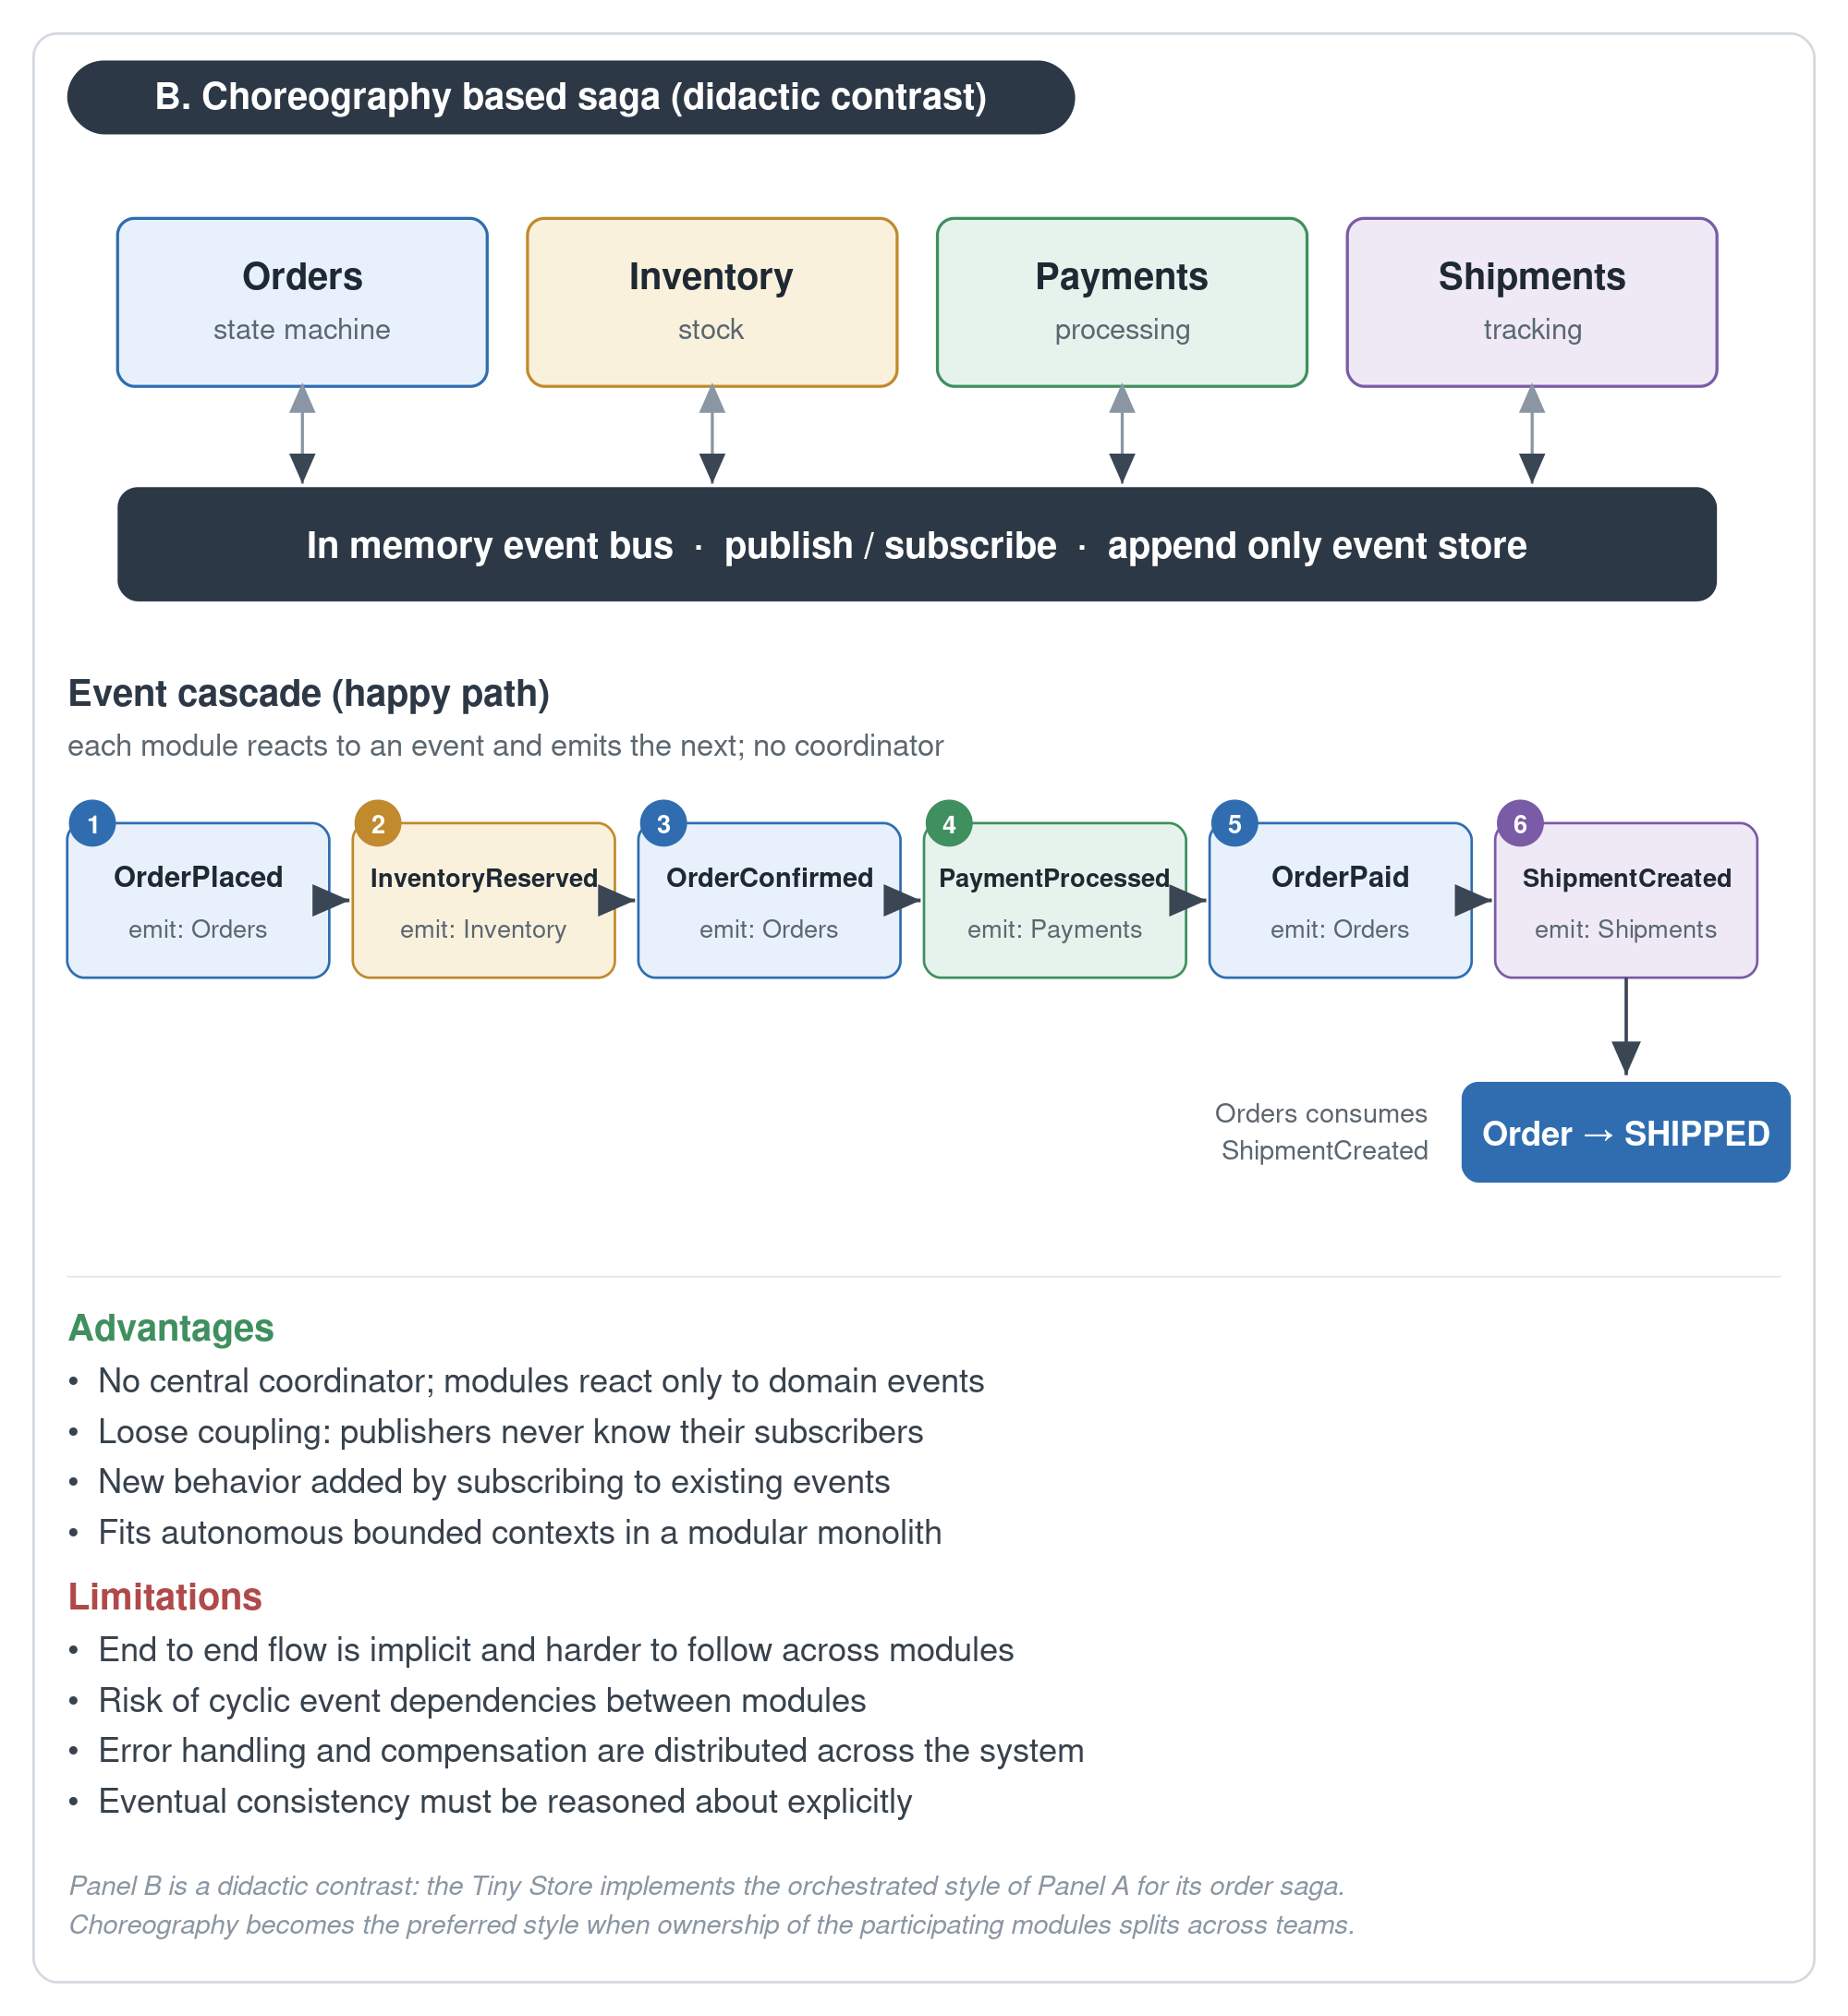
\includegraphics[width=\linewidth]{Cap4/guidelines/saga_pattern_B.png}
  \caption{Choreographed saga style over the same four bounded contexts}
  \label{fig:saga-choreographed}
\end{figure}

\subsubsection*{Comparison}

Table~\ref{tab:saga-styles} consolidates the contrast across eight dimensions relevant to modular monolith adoption, adapted from Newman~\cite{newman2019monolith}. The table is a compact reference for the prose discussion above; readers familiar with both styles can use it as a checklist when characterizing a candidate workflow.

\begin{table}[H]
  \centering
  \small
  \caption{Orchestrated and choreographed saga coordination styles}
  \label{tab:saga-styles}
  \begin{tabularx}{\linewidth}{p{0.22\linewidth} X X}
    \toprule
    \textbf{Dimension} & \textbf{Orchestrated} & \textbf{Choreographed} \\
    \midrule
    Control flow & Centralized & Distributed \\
    Coordinator & Workflow engine (Temporal) & Event bus \\
    Workflow visibility & One file & Across subscribers \\
    Failure handling & Orchestrator-owned & Per-participant \\
    Coupling & Orchestrator to all participants & Shared event schemas only \\
    Team topology & Single team & Multiple teams \\
    State ownership & Central & Distributed \\
    Adding a step & Change orchestrator & Add subscriber \\
    \bottomrule
  \end{tabularx}
\end{table}

\subsubsection*{Trade-offs in practice}

Neither saga style is universally better; the trade-off is rarely captured along a single dimension. The orchestrated saga trades distributed clarity for centralized accountability, making the workflow easy to read but the orchestrator harder to grow. The choreographed saga trades centralized clarity for distributed autonomy, making participants easy to evolve independently but the end-to-end flow harder to follow. Both costs are visible in the literature and both can be operated by a capable team. The decision is therefore not technical in the strict sense but situational, governed by the team topology and the volatility of the contracts that participants share. The application of this situational choice to the Tiny Store is developed in G4 Applied as a design exercise.
